
\documentclass[11pt,german,hideothersubsections]{beamer}\usepackage[]{graphicx}\usepackage[]{color}
%% maxwidth is the original width if it is less than linewidth
%% otherwise use linewidth (to make sure the graphics do not exceed the margin)
\makeatletter
\def\maxwidth{ %
  \ifdim\Gin@nat@width>\linewidth
    \linewidth
  \else
    \Gin@nat@width
  \fi
}
\makeatother

\definecolor{fgcolor}{rgb}{0.345, 0.345, 0.345}
\newcommand{\hlnum}[1]{\textcolor[rgb]{0.686,0.059,0.569}{#1}}%
\newcommand{\hlstr}[1]{\textcolor[rgb]{0.192,0.494,0.8}{#1}}%
\newcommand{\hlcom}[1]{\textcolor[rgb]{0.678,0.584,0.686}{\textit{#1}}}%
\newcommand{\hlopt}[1]{\textcolor[rgb]{0,0,0}{#1}}%
\newcommand{\hlstd}[1]{\textcolor[rgb]{0.345,0.345,0.345}{#1}}%
\newcommand{\hlkwa}[1]{\textcolor[rgb]{0.161,0.373,0.58}{\textbf{#1}}}%
\newcommand{\hlkwb}[1]{\textcolor[rgb]{0.69,0.353,0.396}{#1}}%
\newcommand{\hlkwc}[1]{\textcolor[rgb]{0.333,0.667,0.333}{#1}}%
\newcommand{\hlkwd}[1]{\textcolor[rgb]{0.737,0.353,0.396}{\textbf{#1}}}%

\usepackage{framed}
\makeatletter
\newenvironment{kframe}{%
 \def\at@end@of@kframe{}%
 \ifinner\ifhmode%
  \def\at@end@of@kframe{\end{minipage}}%
  \begin{minipage}{\columnwidth}%
 \fi\fi%
 \def\FrameCommand##1{\hskip\@totalleftmargin \hskip-\fboxsep
 \colorbox{shadecolor}{##1}\hskip-\fboxsep
     % There is no \\@totalrightmargin, so:
     \hskip-\linewidth \hskip-\@totalleftmargin \hskip\columnwidth}%
 \MakeFramed {\advance\hsize-\width
   \@totalleftmargin\z@ \linewidth\hsize
   \@setminipage}}%
 {\par\unskip\endMakeFramed%
 \at@end@of@kframe}
\makeatother

\definecolor{shadecolor}{rgb}{.97, .97, .97}
\definecolor{messagecolor}{rgb}{0, 0, 0}
\definecolor{warningcolor}{rgb}{1, 0, 1}
\definecolor{errorcolor}{rgb}{1, 0, 0}
\newenvironment{knitrout}{}{} % an empty environment to be redefined in TeX

\usepackage{alltt}

\usepackage{hyperref}
\usepackage{amsmath,nicefrac,booktabs,mathabx}
\usepackage{natbib}
\usepackage{url}
\usepackage{textpos}
\usepackage{listings}
\definecolor{Rblau}{rgb}{.3,.6,.9}

\lstset{language=R,
        basicstyle=\ttfamily\footnotesize,
        keywordstyle=\color{blue}\bfseries,
        identifierstyle=\color{Rblau},
        commentstyle=\color{gray},
        stringstyle=\color{green}\ttfamily,
        showstringspaces=false,
        frame=tb}



\bibpunct{(}{)}{;}{a}{,}{,}
\usepackage[english]{babel}
\usepackage[latin1]{inputenc}
\usepackage{helvet}
\usepackage{graphicx}
\usepackage{color}
\usepackage{multirow,dcolumn}
\usepackage{ragged2e}
\usepackage{xcolor}
\usepackage{colortbl}
\usepackage{tikz}
\usetikzlibrary{calc}
\usepackage{booktabs}
\colorlet{tablesubheadcolor}{gray!25}
\colorlet{tableheadcolor}{gray!40}
\colorlet{tablerowcolor}{gray!15.0}
\usetheme[english]{Gesis}
\setbeamertemplate{navigation symbols}{}
\setbeamertemplate{footline}[frame number]%{\hspace*{.2cm}\insertframenumber}
\setbeamerfont{caption}{size=\footnotesize}
\usefonttheme[onlylarge]{structuresmallcapsserif} % alte Schrift

\newcommand{\R}[1]{{\tt \color{blue}  #1}}
\newtheorem{thm}{Theorem}
\newtheorem{rem}{Bemerkung}
\newtheorem{lem}{Lemma}

\definecolor{hellgrau}{rgb}   {0.109375,  0.40625,   0.51953125}
\definecolor{dunkelgrau}{rgb} {0.009375,  0.30625,   0.41953125}
\definecolor{dunkelgrau2}{rgb}{0.009375,  0.20625,   0.31953125}
\definecolor{hellbraun}{rgb}  {0.9140625, 0.8984375, 0.8046875}
\definecolor{hellbraun2}{rgb} {.95,       0.9,       0.8}
\definecolor{alertred}{rgb}   {0.8515625, 0.3828125, 0.08984375}
\definecolor{orange}{rgb}{1,0.5,0}


\setbeamercolor{firstsecslide}{fg=white,bg=dunkelgrau}
\setbeamertemplate{blocks}[rounded][shadow=true]

\newcolumntype{d}[0]{D{,}{.}{6}}

\newenvironment{itemizeol}{\begin{itemize}[<+->]}{\end{itemize}}
\newenvironment{descriptionol}{\begin{description}[<+->]}{\end{description}}

\newcolumntype{V}[1]{%
  >{\RaggedRight\hspace{0pt}}p{#1}%
}

\newcommand{\emphred}[1]{\textcolor{alertred}{#1}}
\newcommand{\emphcol}[1]{\textcolor{dunkelgrau}{\slshape #1}}

\setcounter{tocdepth}{1}
\setbeamercolor*{section in toc}{fg=hellgrau}
\setbeamertemplate{bibliography item}[default]
\makeatother
\addtobeamertemplate{frametitle}{}{%
\begin{textblock*}{100mm}(.91\textwidth,-1cm)

\includegraphics[height=1cm,width=2cm]{../../../common/pics/GESIS_Logo_kompakt_en.jpg}
\end{textblock*}}
\title[Day 1]{Tutorial: Sampling, Weighting and Estimation\\ \Large{Part 1} }
%\subtitle{Umgang am Beispiel von Telefonstichproben}

\author[M. Sand]{Stefan Zins, Matthias Sand\\ and Jan-Philipp Kolb\\ \vspace{.5cm} \footnotesize{GESIS - Leibniz Institute\\ for the Social Sciences}}
%\institute{\includegraphics[width=4.5cm]{GESIS_Logo_informell}}
\date[]{\color{dunkelgrau}\footnotesize}
% \begin{minipage}{8cm}%
% \begin{center}%
% \scriptsize{
% \textbf{GESIS Summer School}\\ \tiny{Cologne, Germany}%
% }\\
% \vspace{0.25cm}
% \textbf{August 24th, 2015}%
% 
% \end{center}%
% \end{minipage}}%
\IfFileExists{upquote.sty}{\usepackage{upquote}}{}
\begin{document}

\maketitle



%%%%%%%%%%%%%%%%%%%%%%%%presentation%%%%%%%%%%%%%%%%%%%%%%%%%

\begin{frame}[fragile]{Why R?}
%\frametitle{\vspace{-.05cm}\begin{center}Why R?\end{center}}
\begin{itemize}
\item Open Source 
\vspace{.25cm}
\item You can work with several datasets at the same time
\vspace{.25cm}
\item You can create your own objects, functions and packages
\vspace{.25cm}
\item Over 5,000 packages contributed by users available on CRAN
\vspace{.25cm}
\item[$\rightarrow$] Rapid implementation of new (scientific) developments
\vspace{.25cm}
\item[$\rightarrow$] Quick development of new tools that fit the user's demand
\end{itemize}
\end{frame}
%%%%%%%%%%%%%%%%%%%%%%%%%%%%%%%%%%%%%%%%%%%%%%%%%%%%%%%%%%%%%%%%%%%
\begin{frame}[fragile]{Getting Started - Download R}
%\frametitle{\vspace{-.05cm}\begin{center}\footnotesize{Getting Started - Download R}\end{center}}
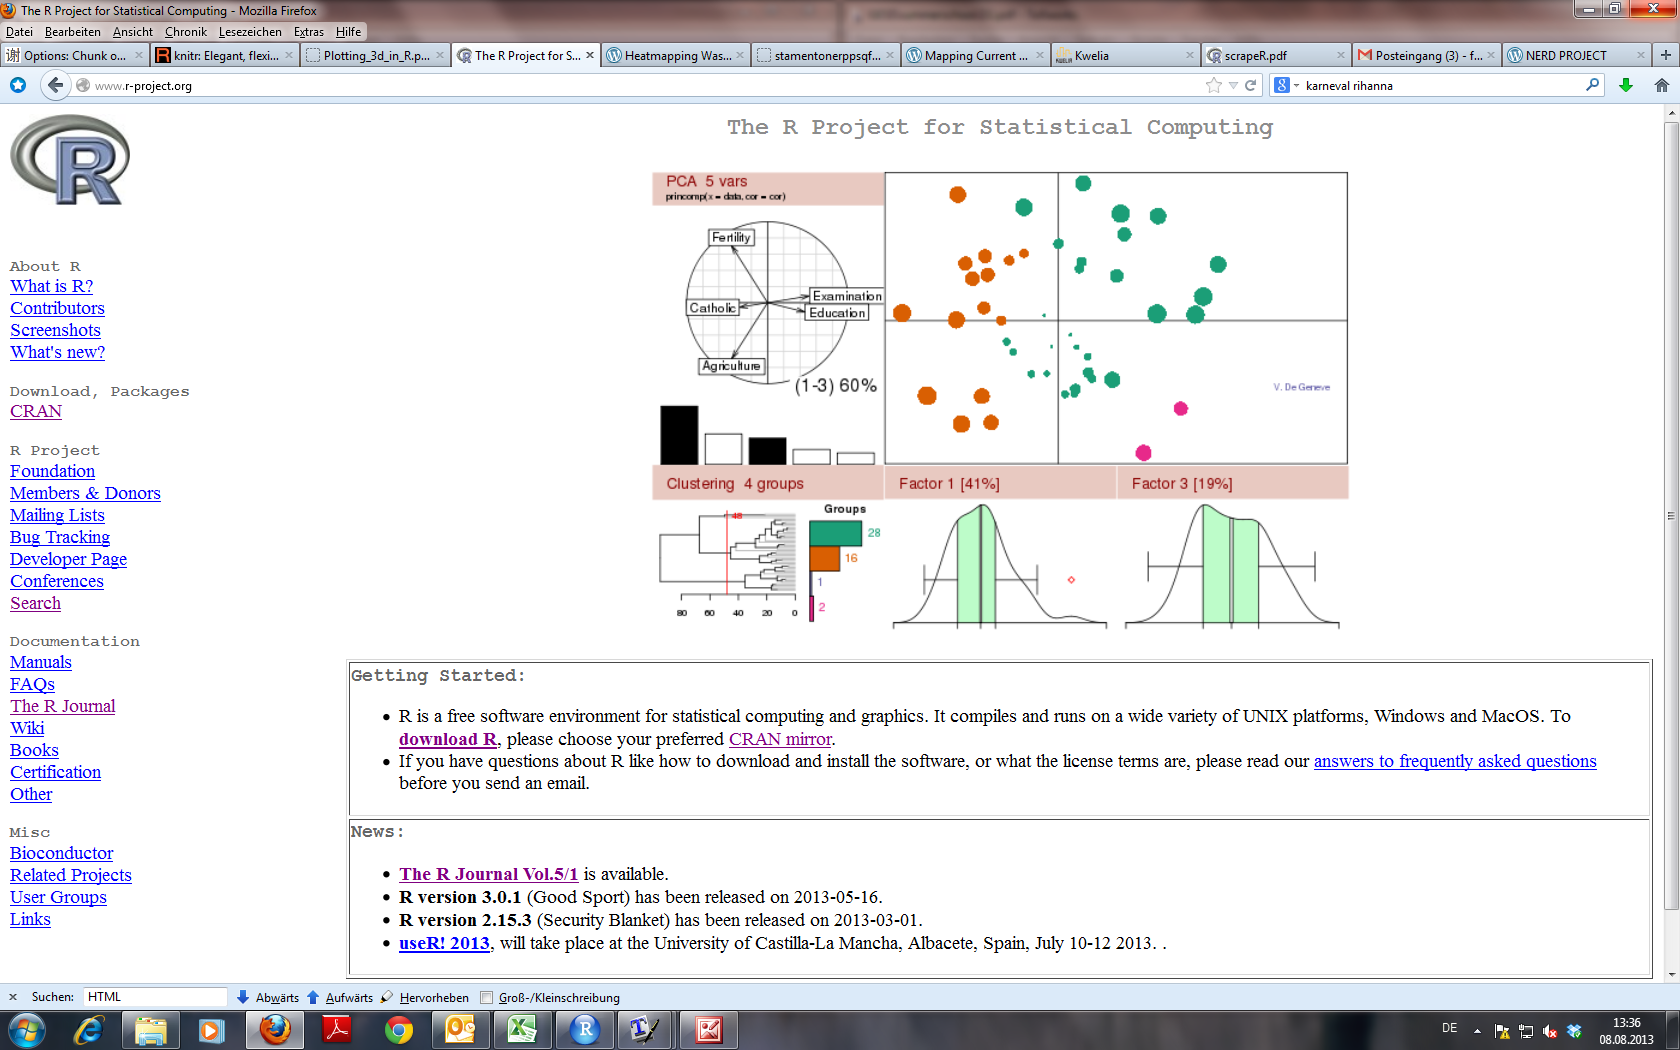
\includegraphics[width=\linewidth, height=6cm]{../../../tutorial/graphs/Rproject.png}
\vspace{.5cm}
\centering
\url{https://www.r-project.org}

\end{frame}
%%%%%%%%%%%%%%%%%%%%%%%%%%%%%%%%%%%%%%%%%%%%%%%%%%%%%%%%%%%%%%%%%%%
\begin{frame}[fragile]{R Basic}
%\frametitle{\vspace{-.05cm}\begin{center}\footnotesize{R Basic}\end{center}}
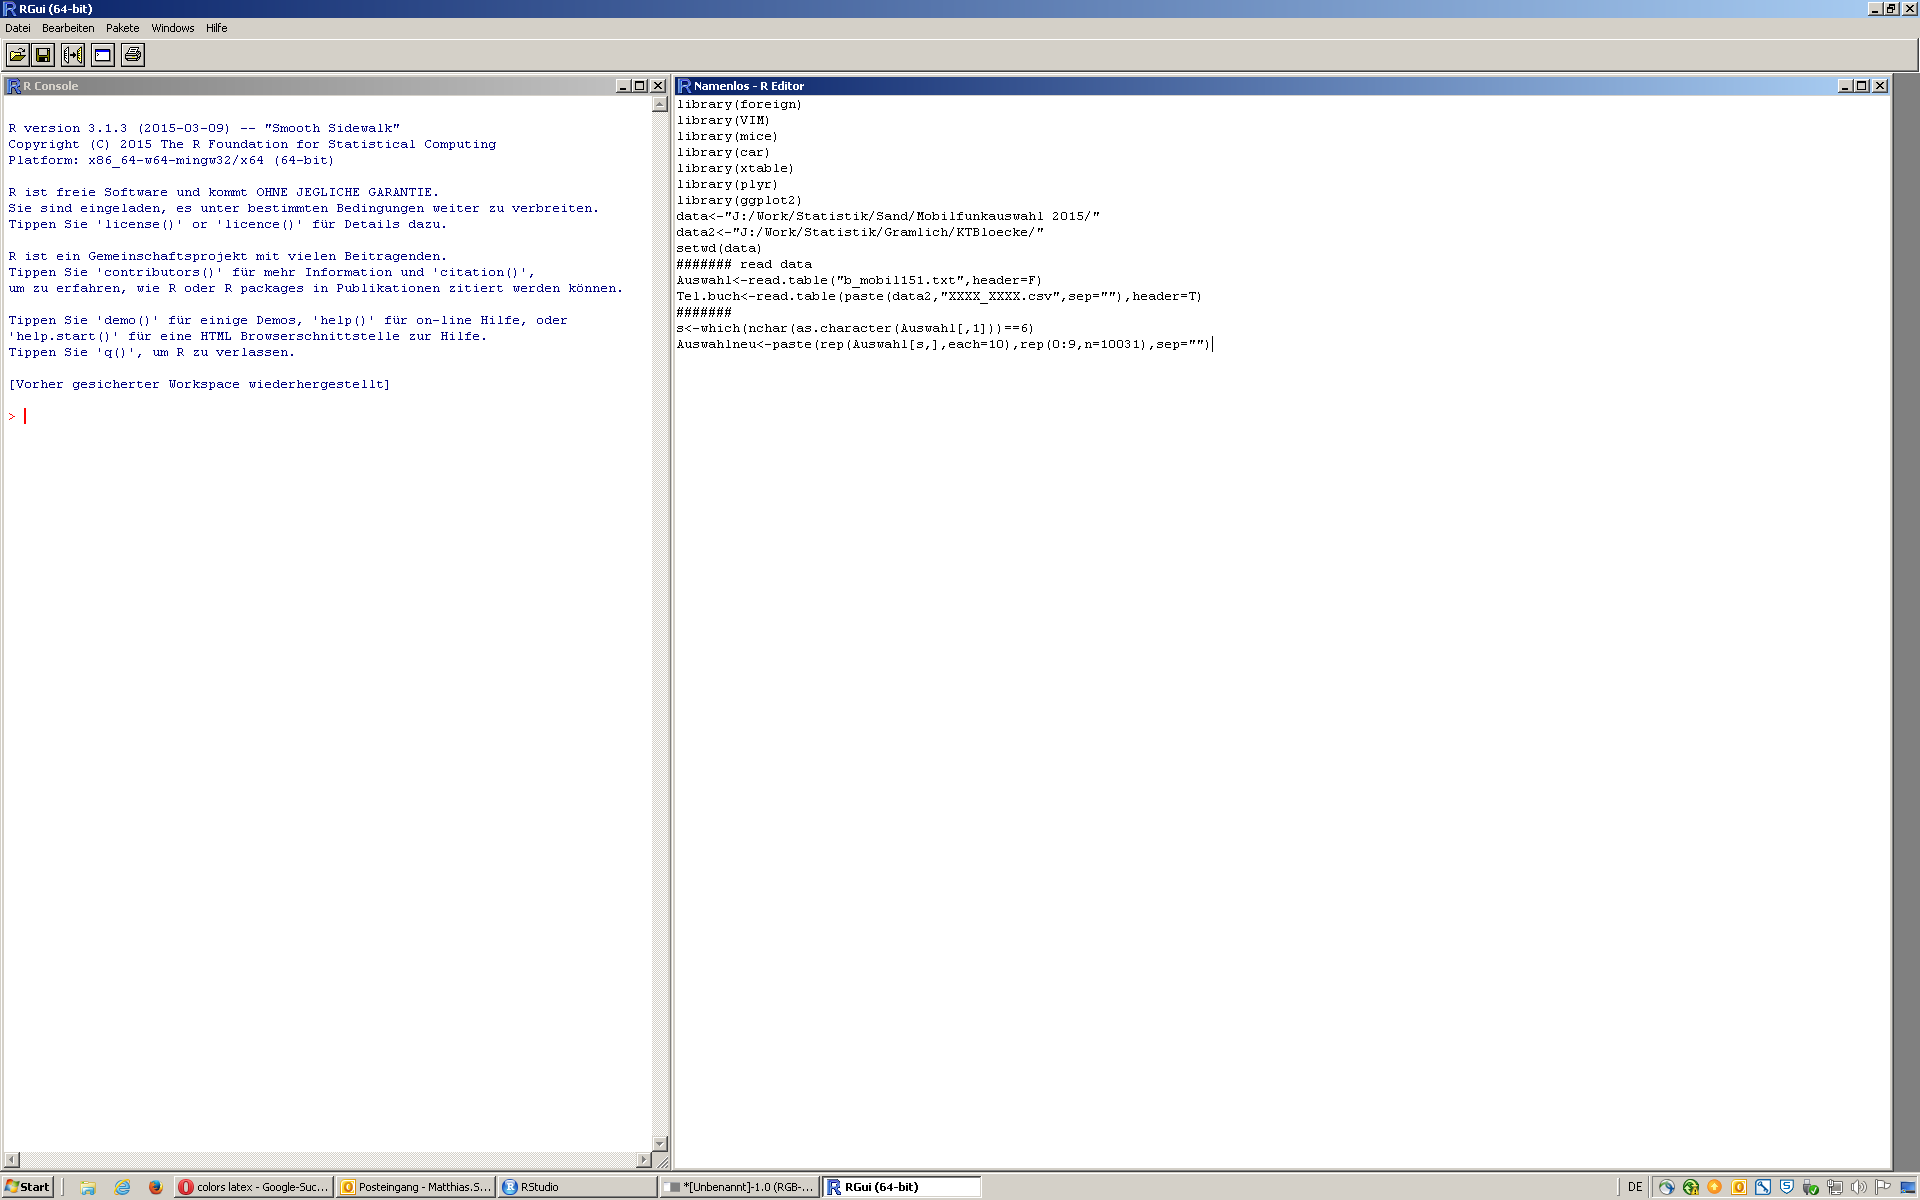
\includegraphics[width=\linewidth, height=6cm]{../../../tutorial/graphs/Ralt.png}
\begin{itemize}
\item most R-user prefer the graphical user interface (GUI) \href{https://www.rstudio.com}{\R{RStudio}}
\end{itemize}
\end{frame}
%%%%%%%%%%%%%%%%%%%%%%%%%%%%%%%%%%%%%%%%%%%%%%%%%%%%%%%%%%%%%%%%%%%%
\begin{frame}[fragile]{R Studio}
%\frametitle{\vspace{-.05cm}\begin{center}\footnotesize{R Studio}\end{center}}
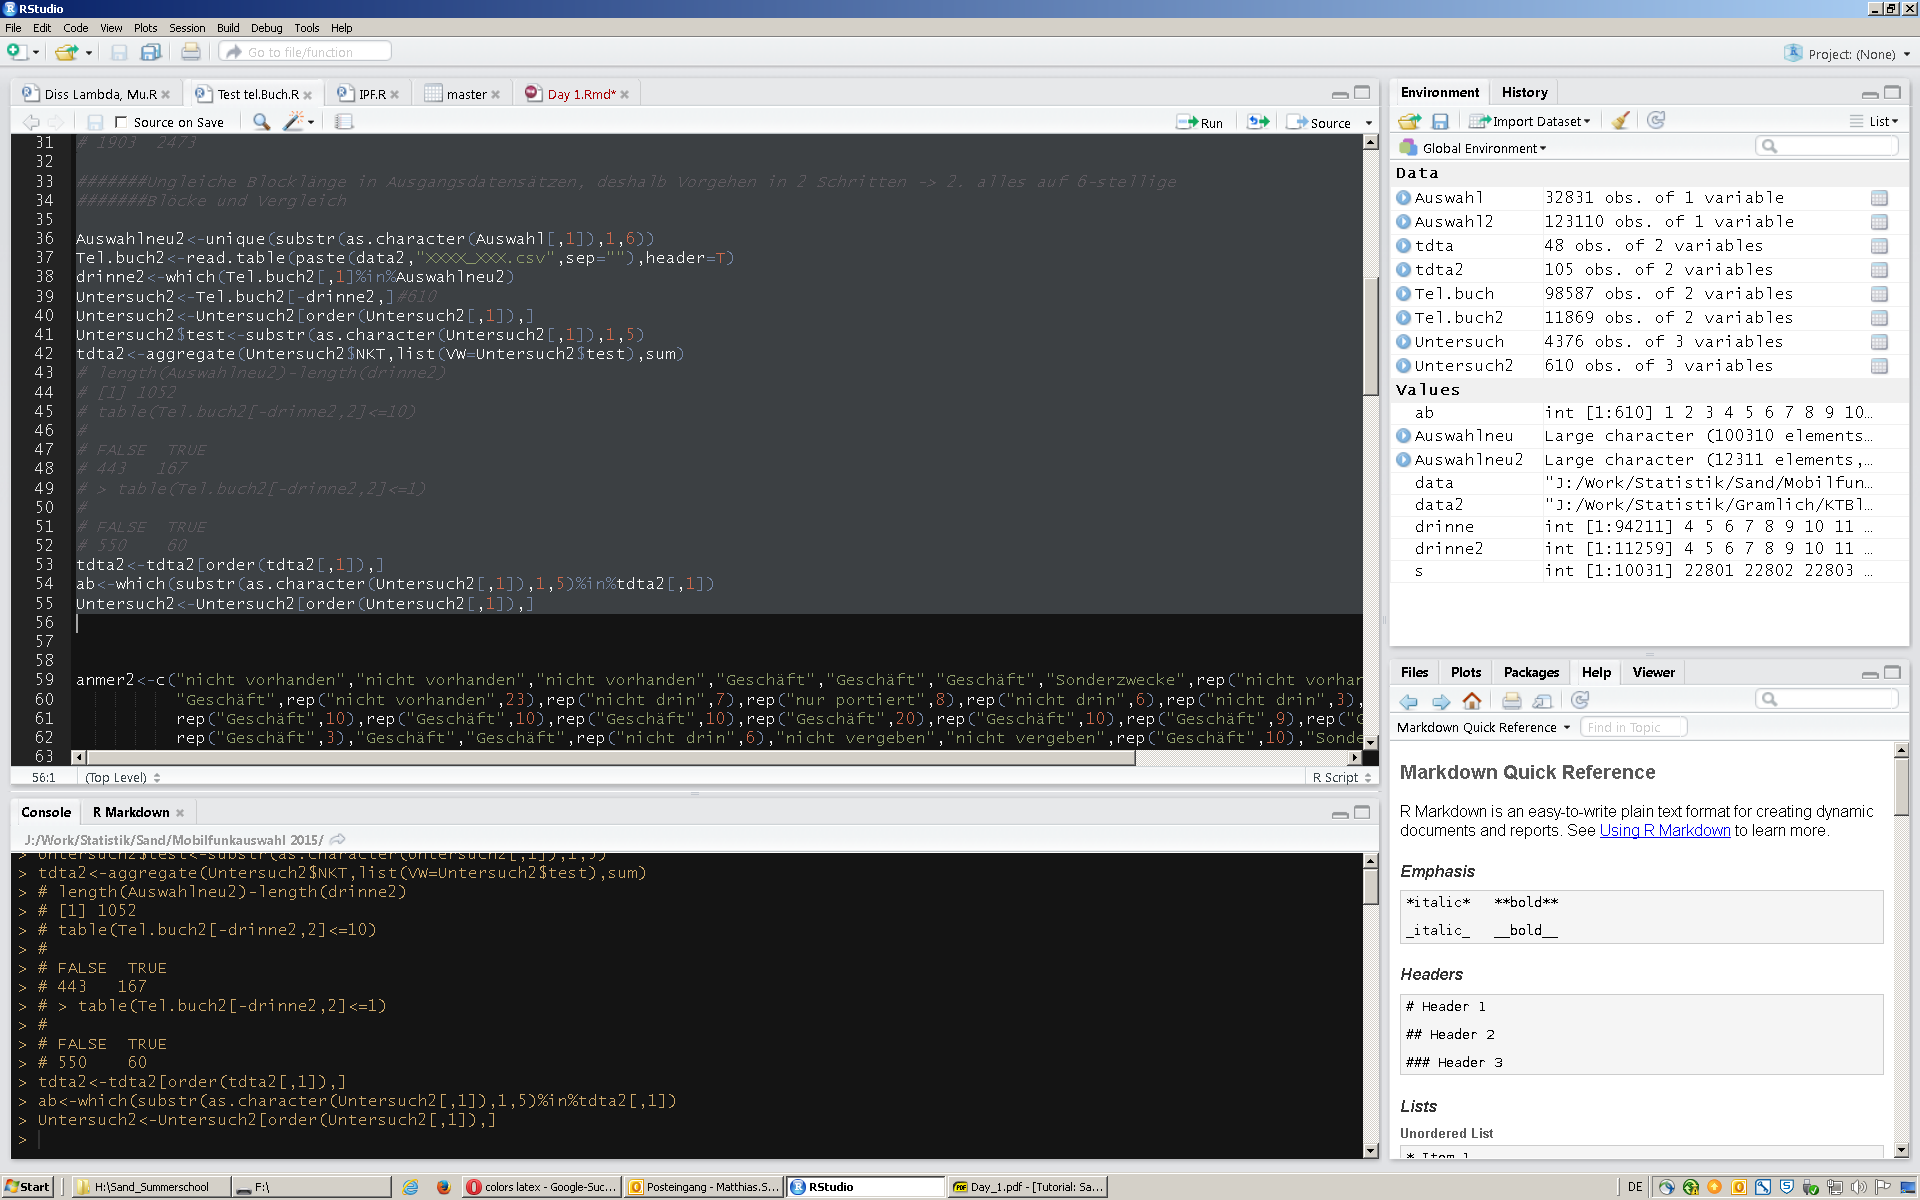
\includegraphics[width=\linewidth, height=6cm]{../../../tutorial/graphs/RStudio.png}
\vspace{.5cm}
\begin{center}
\url{https://www.rstudio.com}
\end{center}
\end{frame}
%%%%%%%%%%%%%%%%%%%%%%%%%%%%%%%%%%%%%%%%%%%%%%%%%%%%%%%%%%%%%%%%%%%%
\begin{frame}[fragile]{Basic R Commands}
%\frametitle{\vspace{-.05cm}\begin{center}\footnotesize{Basic R Commands}\end{center}}
\begin{itemize}
\item \R{<-}  assignment operator
\item \R{\#} can be used to comment your script
\item \R{x<-rnorm(10,0,1)}  creates a vector with ten standardnormal-distributed values
\item \R{mean(x)} calculates the mean of variable \R{x}; \R{length(x)} returns the number of observations in \R{x}
\end{itemize}

\begin{knitrout}
\definecolor{shadecolor}{rgb}{0.969, 0.969, 0.969}\color{fgcolor}\begin{kframe}
\begin{alltt}
\hlkwd{mean}\hlstd{(x)}
\end{alltt}
\begin{verbatim}
## [1] -0.05681029
\end{verbatim}
\begin{alltt}
\hlkwd{length}\hlstd{(x)}
\end{alltt}
\begin{verbatim}
## [1] 10
\end{verbatim}
\end{kframe}
\end{knitrout}
\end{frame}
%%%%%%%%%%%%%%%%%%%%%%%%%%%%%%%%%%%%%%%%%%%%%%%%%%%%%%%%%%%%%%%%%%%%%
\begin{frame}[fragile]{Getting Help}
%\frametitle{\vspace{-.05cm}\begin{center}\footnotesize{Getting Help}\end{center}}
\begin{itemize}
\item \R{?\emph{command}}
\end{itemize}
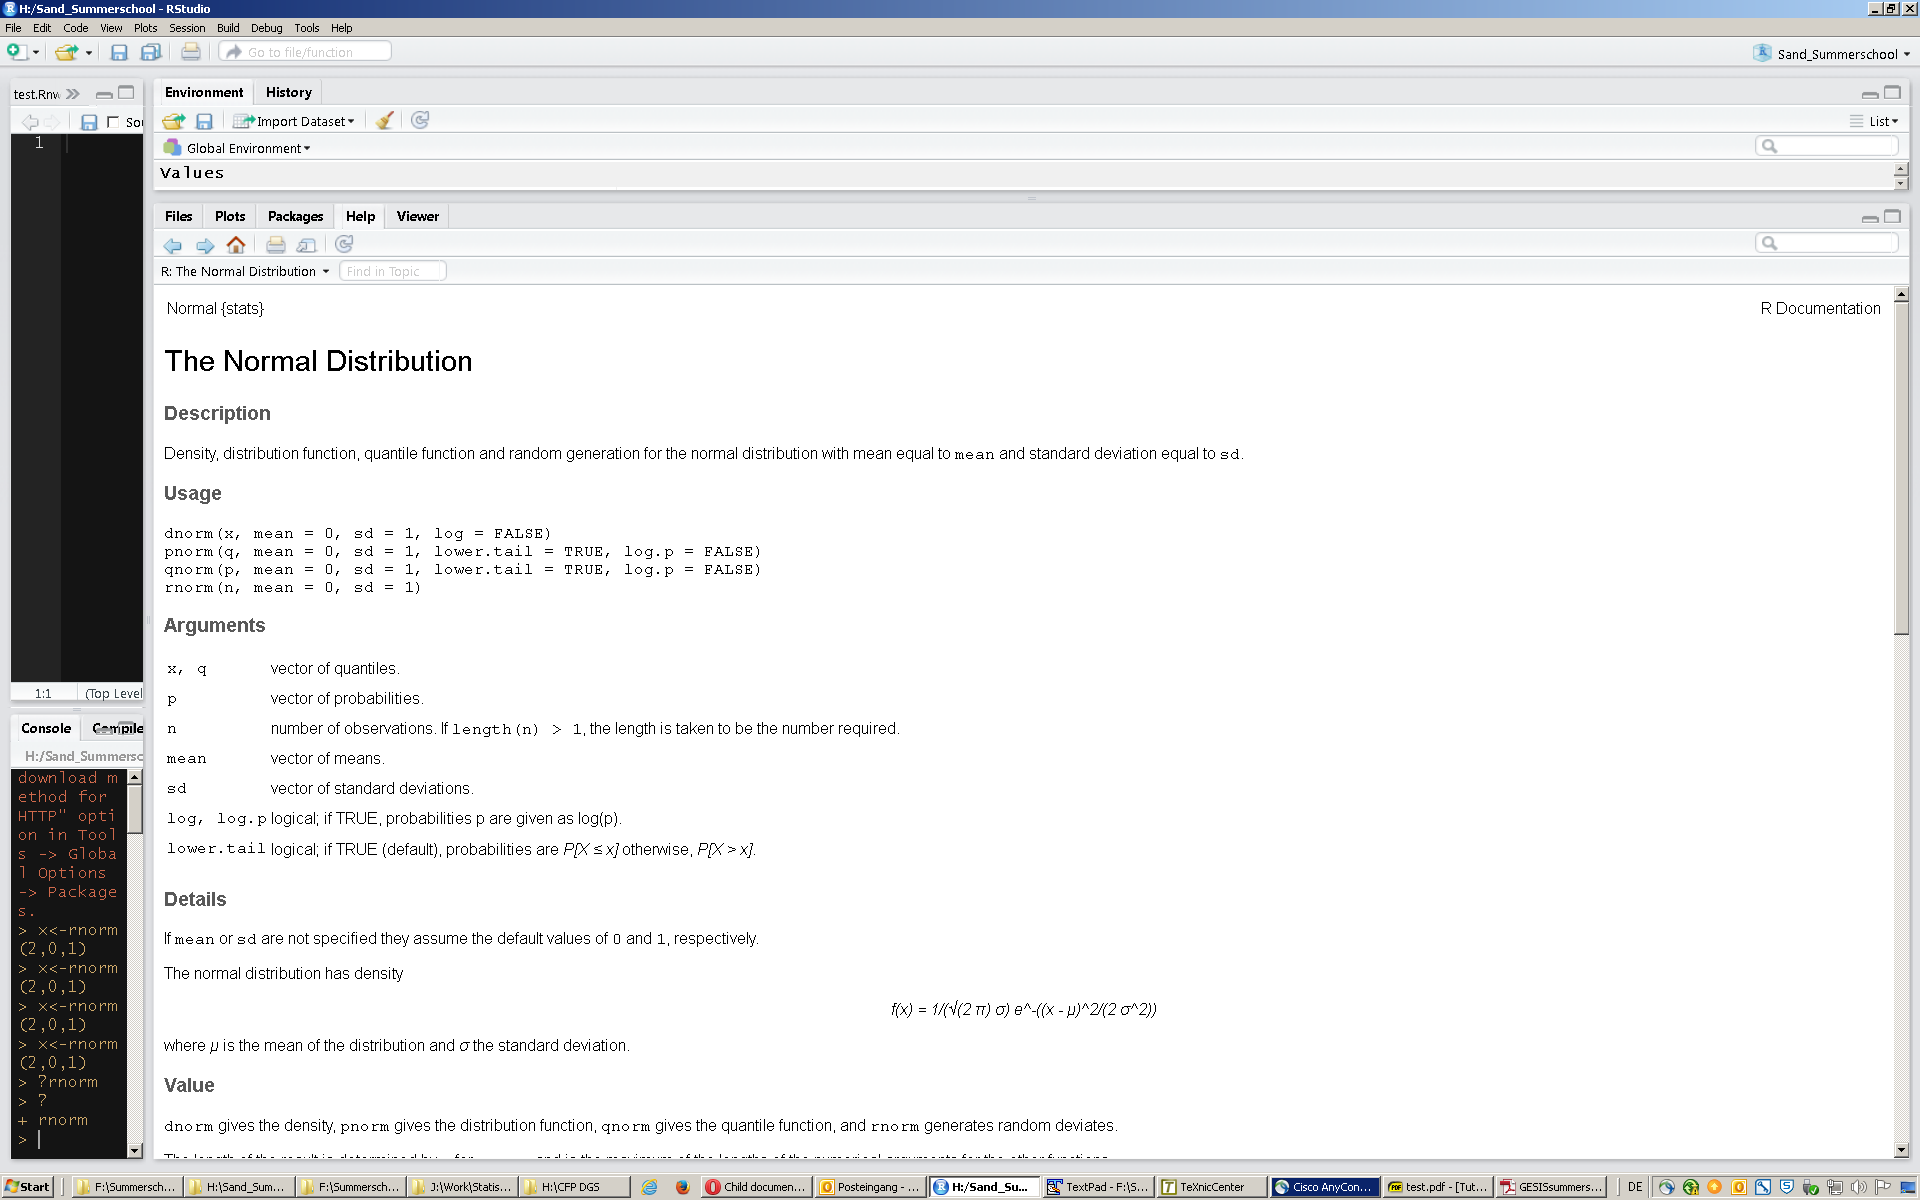
\includegraphics[width=\textwidth, height=4cm]{../../../tutorial/graphs/rhlep.png}
\begin{itemize}
\item \href{https://cran.r-project.org}{CRAN}
\item \href{http://www.statmethods.net}{Quick-R}
\item \href{http://stackoverflow.com/questions/tagged/r}{stackoverflow.com}
\end{itemize}

\end{frame}
%%%%%%%%%%%%%%%%%%%%%%%%%%%%%%%%%%%%%%%%%%%%%%%%%%%%%%%%%%%%%%%%%%%%%%%%%
\begin{frame}[fragile]{Types of Data}
%\frametitle{\vspace{-.05cm}\begin{center}\footnotesize{Types of Data}\end{center}}
\begin{tabular}{l l}
numeric & \R{x<-c(1,2)}\\
logical & \R{x<-c(T,F)}\\
character & \R{x<-c("A","B")}\\
factor & \R{x<-as.factor(c("White","Black"))}\\
\end{tabular}\\
\vspace{.25cm}
\R{str()} returns the type of your data
\begin{knitrout}
\definecolor{shadecolor}{rgb}{0.969, 0.969, 0.969}\color{fgcolor}\begin{kframe}
\begin{alltt}
\hlstd{x}\hlkwb{<-}\hlkwd{as.factor}\hlstd{(}\hlkwd{c}\hlstd{(}\hlstr{"White"}\hlstd{,}\hlstr{"Black"}\hlstd{))}
\hlkwd{str}\hlstd{(x)}
\end{alltt}
\begin{verbatim}
##  Factor w/ 2 levels "Black","White": 2 1
\end{verbatim}
\end{kframe}
\end{knitrout}
\end{frame}
%%%%%%%%%%%%%%%%%%%%%%%%%%%%%%%%%%%%%%%%%%%%%%%%%%%%%%%%%%%%%%%%%%%%%%%%
\begin{frame}[fragile]{Indexing I}
%\frametitle{\vspace{-.05cm}\begin{center}\footnotesize{Indexing I}\end{center}}
\begin{center}
\textbf{Indexing a Vector:}
\end{center}
\begin{knitrout}
\definecolor{shadecolor}{rgb}{0.969, 0.969, 0.969}\color{fgcolor}\begin{kframe}
\begin{alltt}
\hlstd{A1}\hlkwb{<-}\hlkwd{c}\hlstd{(}\hlnum{1}\hlstd{,}\hlnum{2}\hlstd{,}\hlnum{3}\hlstd{,}\hlnum{4}\hlstd{)}
\hlstd{A1[}\hlnum{1}\hlstd{]}
\end{alltt}
\begin{verbatim}
## [1] 1
\end{verbatim}
\begin{alltt}
\hlstd{A1[}\hlnum{1}\hlopt{:}\hlnum{3}\hlstd{]}
\end{alltt}
\begin{verbatim}
## [1] 1 2 3
\end{verbatim}
\begin{alltt}
\hlstd{A1[}\hlopt{-}\hlnum{2}\hlstd{]}
\end{alltt}
\begin{verbatim}
## [1] 1 3 4
\end{verbatim}
\end{kframe}
\end{knitrout}
\end{frame}
%%%%%%%%%%%%%%%%%%%%%%%%%%%%%%%%%%%%%%%%%%%%%%%%%%%%%%%%%%%%%%%%%%%%%%%%%%
\begin{frame}[fragile]{Indexing II}
%\frametitle{\vspace{-.05cm}\begin{center}\footnotesize{Indexing II}\end{center}}
\begin{center}
\textbf{Indexing a data frame:}
\end{center}
\begin{knitrout}
\definecolor{shadecolor}{rgb}{0.969, 0.969, 0.969}\color{fgcolor}\begin{kframe}
\begin{alltt}
\hlstd{A2}\hlkwb{<-}\hlnum{4}\hlopt{:}\hlnum{1}
\hlstd{AA}\hlkwb{<-}\hlkwd{cbind}\hlstd{(A1,A2)}
\hlstd{AA[}\hlnum{1}\hlstd{,]}
\end{alltt}
\begin{verbatim}
## A1 A2 
##  1  4
\end{verbatim}
\begin{alltt}
\hlstd{AA[,}\hlnum{1}\hlstd{]}
\end{alltt}
\begin{verbatim}
## [1] 1 2 3 4
\end{verbatim}
\begin{alltt}
\hlstd{AA[}\hlnum{1}\hlopt{:}\hlnum{3}\hlstd{,}\hlnum{2}\hlstd{]}
\end{alltt}
\begin{verbatim}
## [1] 4 3 2
\end{verbatim}
\begin{alltt}
\hlstd{AA[,}\hlopt{-}\hlnum{1}\hlstd{]}
\end{alltt}
\begin{verbatim}
## [1] 4 3 2 1
\end{verbatim}
\end{kframe}
\end{knitrout}
\end{frame}
%%%%%%%%%%%%%%%%%%%%%%%%%%%%%%%%%%%%%%%%%%%%%%%%%%%%%%%%%%%%%%%%%%%%%%%%%%
\begin{frame}[fragile]{Indexing III}
%\frametitle{\vspace{-.05cm}\begin{center}\footnotesize{Indexing III}\end{center}}
\begin{center}
\textbf{Indexing an array}
\end{center}
\begin{scriptsize}
\begin{knitrout}
\definecolor{shadecolor}{rgb}{0.969, 0.969, 0.969}\color{fgcolor}\begin{kframe}
\begin{alltt}
\hlstd{A3}\hlkwb{<-}\hlkwd{array}\hlstd{(}\hlnum{1}\hlopt{:}\hlnum{8}\hlstd{,}\hlkwd{c}\hlstd{(}\hlnum{2}\hlstd{,}\hlnum{2}\hlstd{,}\hlnum{2}\hlstd{))}
\hlstd{A3}
\end{alltt}
\begin{verbatim}
## , , 1
## 
##      [,1] [,2]
## [1,]    1    3
## [2,]    2    4
## 
## , , 2
## 
##      [,1] [,2]
## [1,]    5    7
## [2,]    6    8
\end{verbatim}
\begin{alltt}
\hlstd{A3[,,}\hlnum{2}\hlstd{]}
\end{alltt}
\begin{verbatim}
##      [,1] [,2]
## [1,]    5    7
## [2,]    6    8
\end{verbatim}
\end{kframe}
\end{knitrout}
\end{scriptsize}
\end{frame}
%%%%%%%%%%%%%%%%%%%%%%%%%%%%%%%%%%%%%%%%%%%%%%%%%%%%%%%%%%%%%%%%%%%%%%%%%%
\begin{frame}[fragile]{Indexing IV}
%\frametitle{\vspace{-.05cm}\begin{center}\footnotesize{Indexing IV}\end{center}}
\begin{center}
\textbf{Indexing a list}
\end{center}
\begin{knitrout}
\definecolor{shadecolor}{rgb}{0.969, 0.969, 0.969}\color{fgcolor}\begin{kframe}
\begin{alltt}
\hlstd{A4}\hlkwb{<-}\hlkwd{list}\hlstd{(A1,}\hlkwd{c}\hlstd{(}\hlstr{"Summer"}\hlstd{,}\hlstr{"Winter"}\hlstd{))}
\hlstd{A4}
\end{alltt}
\begin{verbatim}
## [[1]]
## [1] 1 2 3 4
## 
## [[2]]
## [1] "Summer" "Winter"
\end{verbatim}
\begin{alltt}
\hlstd{A4[[}\hlnum{1}\hlstd{]]}
\end{alltt}
\begin{verbatim}
## [1] 1 2 3 4
\end{verbatim}
\end{kframe}
\end{knitrout}
\end{frame}
%%%%%%%%%%%%%%%%%%%%%%%%%%%%%%%%%%%%%%%%%%%%%%%%%%%%%%%%%%%%%%%%%%%%%%%%%%
\begin{frame}[fragile]{Sequences}
%\frametitle{\vspace{-.05cm}\begin{center}\footnotesize{Sequences}\end{center}}
\begin{knitrout}
\definecolor{shadecolor}{rgb}{0.969, 0.969, 0.969}\color{fgcolor}\begin{kframe}
\begin{alltt}
\hlnum{1}\hlopt{:}\hlnum{5}
\end{alltt}
\begin{verbatim}
## [1] 1 2 3 4 5
\end{verbatim}
\begin{alltt}
\hlkwd{rep}\hlstd{(}\hlstr{"A"}\hlstd{,}\hlkwc{times}\hlstd{=}\hlnum{10}\hlstd{)}
\end{alltt}
\begin{verbatim}
##  [1] "A" "A" "A" "A" "A" "A" "A" "A" "A" "A"
\end{verbatim}
\begin{alltt}
\hlkwd{rep}\hlstd{(}\hlnum{1}\hlopt{:}\hlnum{3}\hlstd{,}\hlkwc{times}\hlstd{=}\hlnum{2}\hlstd{,}\hlkwc{each}\hlstd{=}\hlnum{3}\hlstd{)}
\end{alltt}
\begin{verbatim}
##  [1] 1 1 1 2 2 2 3 3 3 1 1 1 2 2 2 3 3 3
\end{verbatim}
\begin{alltt}
\hlkwd{seq}\hlstd{(}\hlopt{-}\hlnum{5}\hlstd{,}\hlnum{5}\hlstd{,}\hlkwc{by}\hlstd{=}\hlnum{2.5}\hlstd{)}
\end{alltt}
\begin{verbatim}
## [1] -5.0 -2.5  0.0  2.5  5.0
\end{verbatim}
\end{kframe}
\end{knitrout}
\end{frame}
%%%%%%%%%%%%%%%%%%%%%%%%%%%%%%%%%%%%%%%%%%%%%%%%%%%%%%%%%%%%%%%%%%%%%%%%%%%%
\begin{frame}[fragile]{Random Numbers}
%\frametitle{\vspace{-.05cm}\begin{center}\footnotesize{Random Numbers}\end{center}}
\begin{center}
\begin{tabular}{l|l|l}
\textbf{Function } & \textbf{Distribution} & \textbf{Important parameter} \\
\hline
\hline
\R{runif()} & Uniform distribution & n, min, max\\
\hline
\R{rnorm()} & Normal distribution & n, mean, sd \\
\hline
\R{rpois()} & Poisson distribution & n, lambda\\
\hline 
... & ... & ... \\
\end{tabular}
\end{center}
\end{frame}

%%%%%%%%%%%%%%%%%%%%%%%%%%%%%%%%%%%%%%%%%%%%%%%%%%%%%%%%%%%%%%%%%%%%%%%%%%
\begin{frame}[fragile]{Important Functions} {of the \{base\}-Package}
%\frametitle{\vspace{-.05cm}\begin{center}\footnotesize{Important Functions of the \{base\}-Package}\end{center}}
\begin{center}
\renewcommand{\arraystretch}{.75}
\begin{tabular}{lll}
Function & Meaning & Example \\
\hline
\R{length()} & Length & \R{length(x)}\\
\R{max()} & Maximum & \R{max(x)}\\
\R{min()} & Minimum & \R{min(x)}\\
\R{sd()} & Standard deviation & \R{sd(x)}\\
\R{var()} & Variance & \R{var(x)}\\
\R{mean()} & Mean & \R{mean(x)} \\
\R{median()} & Median & \R{median(x)} \\
&& \\
\multicolumn{3}{c}{These functions do only need one argument}\\
\multicolumn{3}{c}{Other functions need to be specified by further arguments:}\\
&& \\
\R{quantile()} & 90\% Quantile & \R{quantile(x,.9)}\\ 
\R{sample()} & Draw a sample & \R{sample(x,1)}\\
\end{tabular}
\end{center}
\begin{itemize}
\pause\item \R{R} is a modular program with many functions included in basic \R{R}
\pause\item more specific functions are embedded in further packages
\end{itemize}
\end{frame}


%%%%%%%%%%%%%%%%%%%%%%%%%%%%%%%%%%%%%%%%%%%%%%%%%%%%%%%%%%%%%%%%%%%%%%%%%%
\begin{frame}[fragile]{Installing and Loading Packages}
%\frametitle{\vspace{-.05cm}\begin{center}\footnotesize{Installing and Loading Packages}\end{center}}
\R{install.package("sampling")}\\
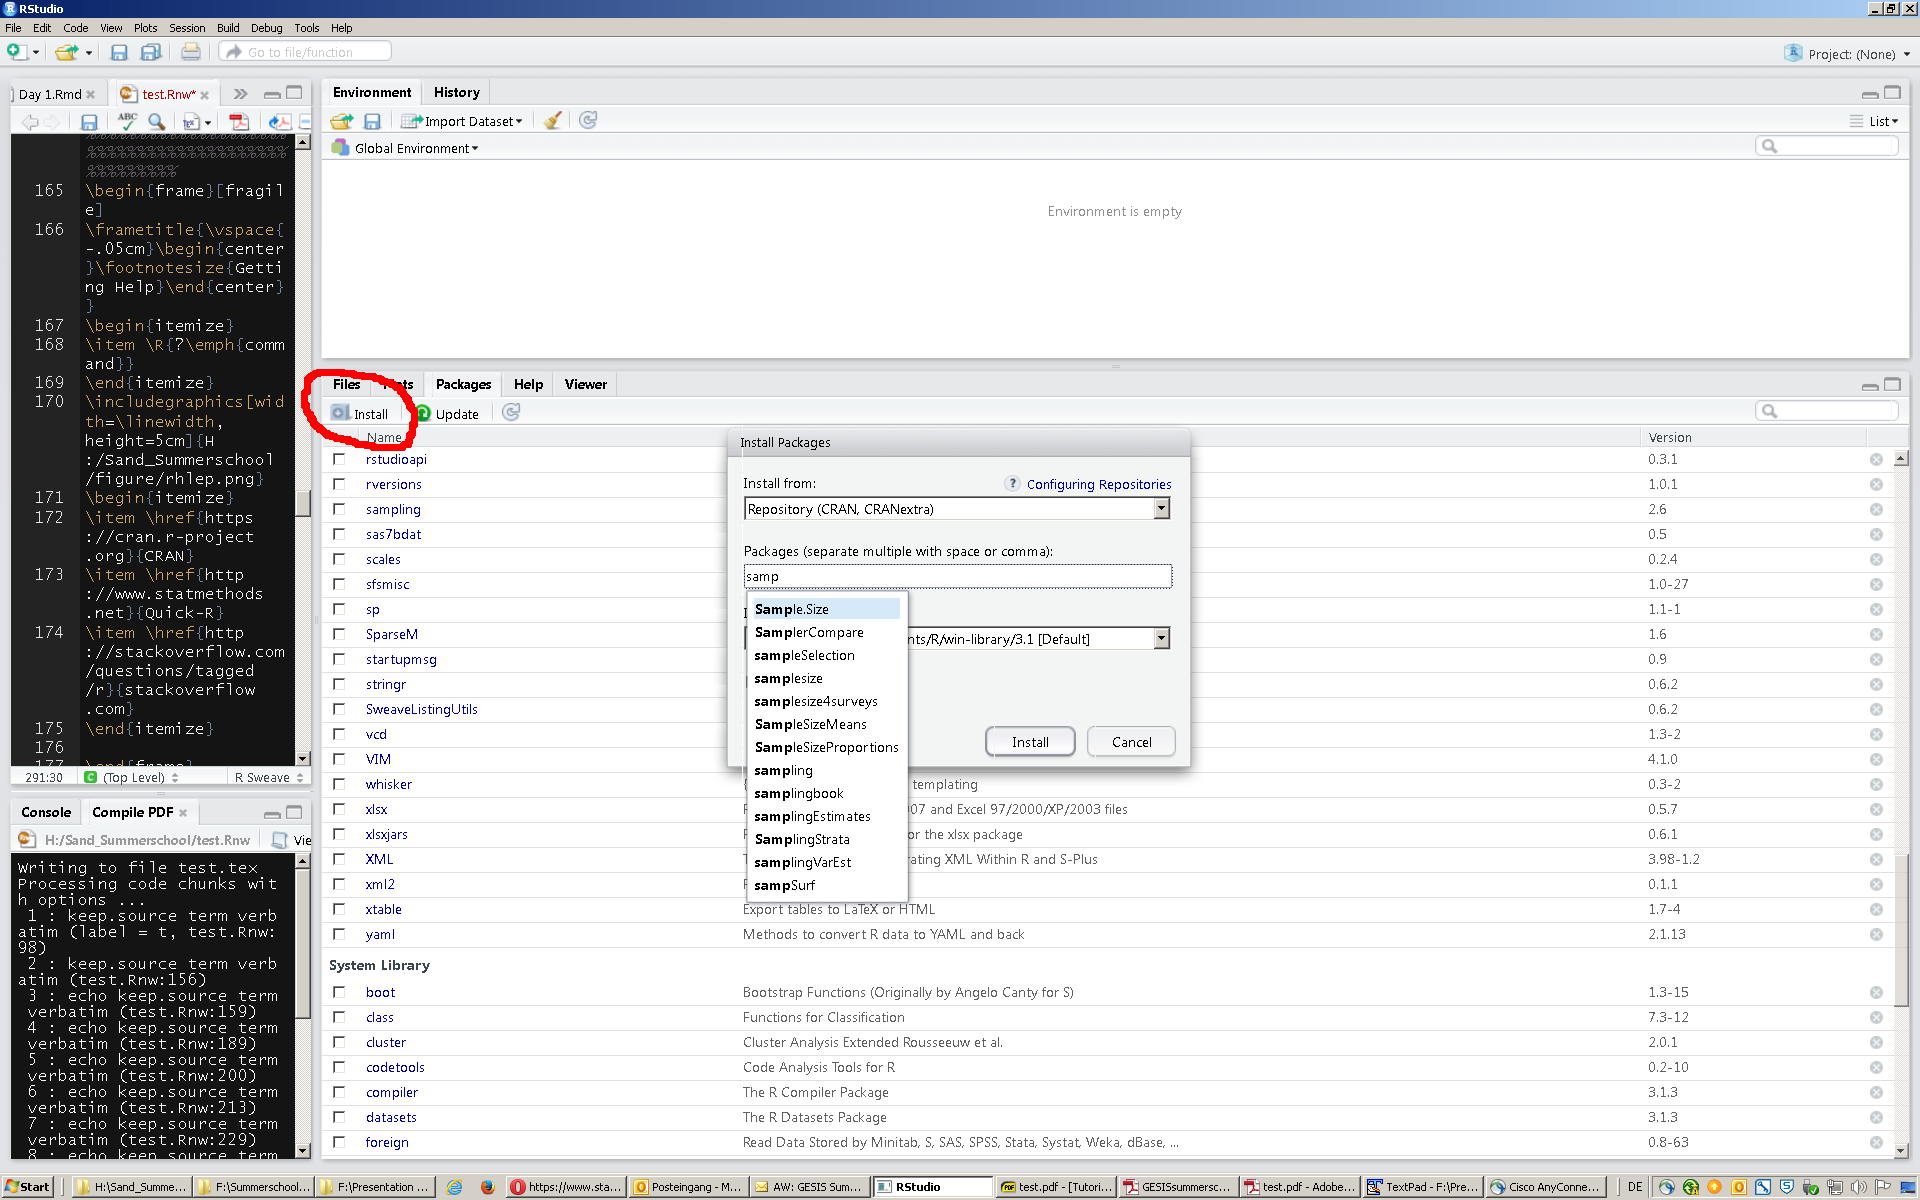
\includegraphics[width=\linewidth, height=5cm]{../../../tutorial/graphs/Rpackages.png}
\vspace{.25cm}
\R{library(sampling)} \emph{or} \R{require(sampling)}
\end{frame}
%%%%%%%%%%%%%%%%%%%%%%%%%%%%%%%%%%%%%%%%%%%%%%%%%%%%%%%%%%%%%%%%%%%%%%%%%%
\begin{frame}[fragile]{Useful Packages}
%\frametitle{\vspace{-.05cm}\begin{center}\footnotesize{Useful Packages}\end{center}}
\renewcommand{\arraystretch}{1}
\begin{tabular}{l|l}
Library & Subject\\
\hline
\R{foreign} & reading and writing of data in\\ 
& numerous formats (e.g. \emph{.dta}, \emph{.sav})\\
\R{sampling} & drawing and weighting samples\\
\R{survey} & analysis of complex survey samples\\
\R{xlsx} & read and write data in Excell-Format\\
\R{xtable} & export tables to LaTex and HTML\\
\R{mice} & multiple imputation by chain equation\\
\R{reshape} & alter structure of datasets\\
\R{car} & applied regressions\\
\R{VIM} & visualization and imputation of Missing Values\\
\R{lattice} & high-level data visualization\\
\R{ggplot2} & grammar for graphics in \R{R}\\
\end{tabular}
\end{frame}
%%%%%%%%%%%%%%%%%%%%%%%%%%%%%%%%%%%%%%%%%%%%%%%%%%%%%%%%%%%%%%%%%%%%%%%%%%
\begin{frame}[fragile]{Basic Graphics}
%\frametitle{\vspace{-.05cm}\begin{center}\footnotesize{Basic Graphics}\end{center}}

\begin{columns}
\begin{column}{.5\textwidth}
\begin{knitrout}
\definecolor{shadecolor}{rgb}{0.969, 0.969, 0.969}\color{fgcolor}\begin{kframe}
\begin{alltt}
\hlkwd{set.seed}\hlstd{(}\hlnum{42}\hlstd{)}
\hlstd{x} \hlkwb{<-} \hlkwd{rnorm}\hlstd{(}\hlnum{1000}\hlstd{,}\hlnum{0}\hlstd{,}\hlnum{1}\hlstd{)}
\hlkwd{plot}\hlstd{(x)}
\end{alltt}
\end{kframe}
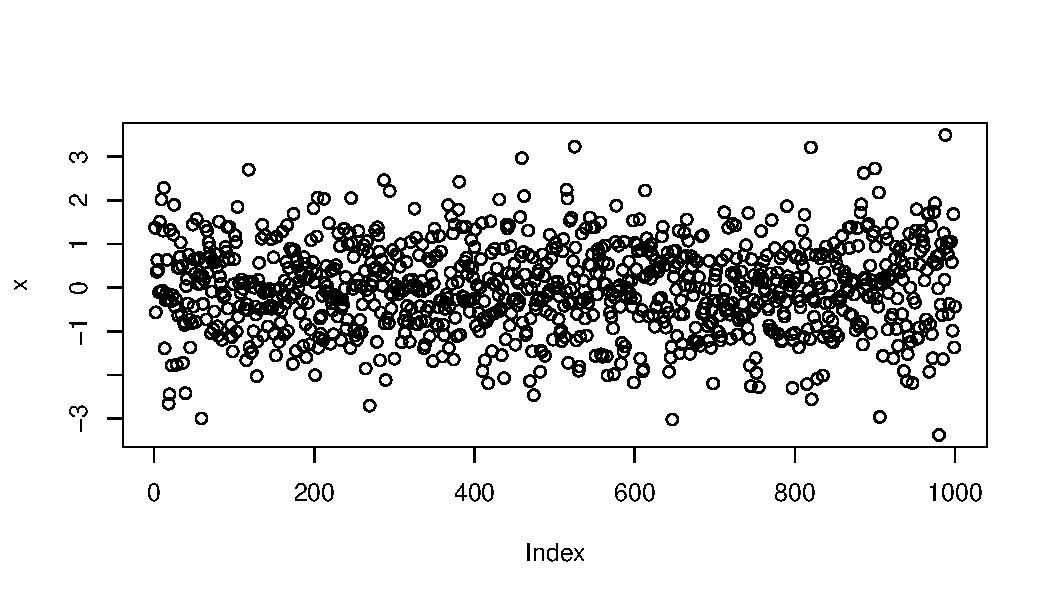
\includegraphics[width=\maxwidth]{figure/unnamed-chunk-9-1} 

\end{knitrout}
\end{column}
\vspace{.25cm}
\begin{column}{.5\textwidth}

\R{set.seed()} is used to specify a starting point

\begin{knitrout}
\definecolor{shadecolor}{rgb}{0.969, 0.969, 0.969}\color{fgcolor}\begin{kframe}
\begin{alltt}
\hlkwd{hist}\hlstd{(x)}
\end{alltt}
\end{kframe}
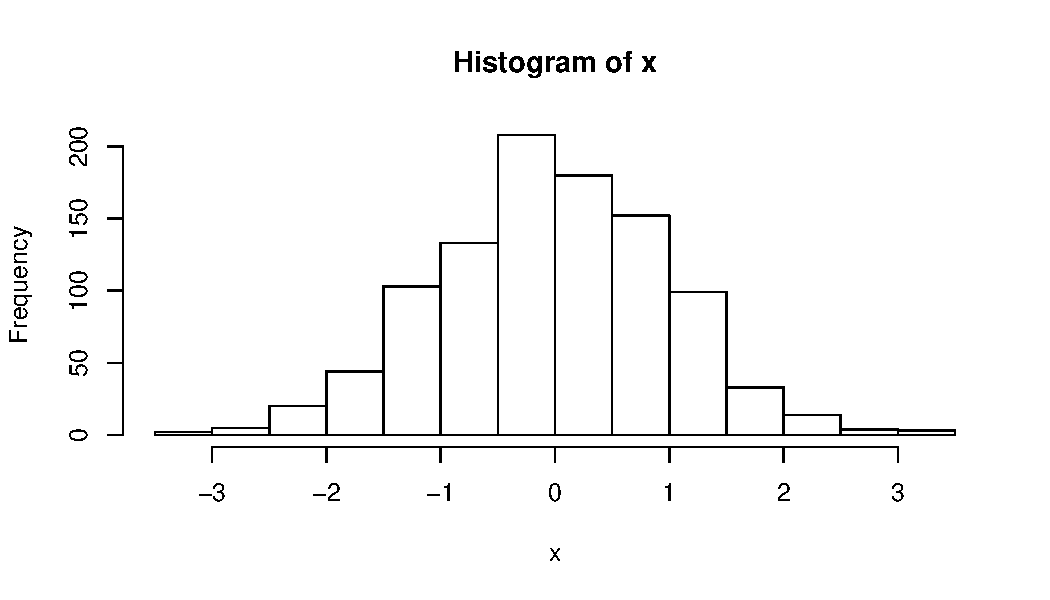
\includegraphics[width=\maxwidth]{figure/unnamed-chunk-10-1} 

\end{knitrout}
\end{column}
\end{columns}
\begin{itemize}
\item[$\Rightarrow$] we will use \emph{42} as seed-value for future exercises to obtain comparable results
\end{itemize}
\end{frame}
%%%%%%%%%%%%%%%%%%%%%%%%%%%%%%%%%%%%%%%%%%%%%%%%%%%%%%%%%%%%%%%%%%%%%%%%%%
\begin{frame}[fragile]{The Basic \R{sample} Function}
%\frametitle{\vspace{-.05cm}\begin{center}\footnotesize{The Basic \R{sample} Function}\end{center}}
\begin{center}
\pgfdeclareimage[width=.6\textwidth]{SampleHelp}{../../../tutorial/graphs/SampleHelp.PNG}
\pgfuseimage{SampleHelp}

\pgfdeclareimage[width=.6\textwidth]{SampleWhat}{../../../tutorial/graphs/SampleWhat2.PNG}
\pgfdeclareimage[width=.6\textwidth]{SampleHow}{../../../tutorial/graphs/SampleHow.PNG}
\pgfdeclareimage[width=.6\textwidth]{SampleReplacement}{../../../tutorial/graphs/SampleReplacement.PNG}

\pgfuseimage<1>{SampleWhat}
\pgfuseimage<2>{SampleHow}
\pgfuseimage<3>{SampleReplacement}

\end{center}
\end{frame}
%%%%%%%%%%%%%%%%%%%%%%%%%%%%%%%%%%%%%%%%%%%%%%%%%%%%%%%%%%%%%%%%%%%%%%%%%%
\begin{frame}[fragile]{Simple Example on Sampling}
%\frametitle{\vspace{-.05cm}\begin{center}\footnotesize{Simple Example on Sampling}\end{center}}
\begin{footnotesize}
\begin{knitrout}
\definecolor{shadecolor}{rgb}{0.969, 0.969, 0.969}\color{fgcolor}\begin{kframe}
\begin{alltt}
\hlstd{id} \hlkwb{<-} \hlnum{1}\hlopt{:}\hlnum{10000}
\hlkwd{set.seed}\hlstd{(}\hlnum{42}\hlstd{)}
\hlstd{education} \hlkwb{<-} \hlkwd{sample}\hlstd{(}\hlkwd{c}\hlstd{(}\hlstr{"none"}\hlstd{,}\hlstr{"low"}\hlstd{,}\hlstr{"average"}\hlstd{,}\hlstr{"high"}\hlstd{),}\hlnum{10000}\hlstd{,}
                    \hlkwc{replace} \hlstd{= T,}\hlkwc{prob} \hlstd{=} \hlkwd{c}\hlstd{(}\hlnum{.072}\hlstd{,}\hlnum{.356}\hlstd{,}\hlnum{.289}\hlstd{,}\hlnum{.283}\hlstd{))}

\hlstd{gender} \hlkwb{<-} \hlkwd{sample}\hlstd{(}\hlkwd{c}\hlstd{(}\hlstr{"male"}\hlstd{,}\hlstr{"female"}\hlstd{),}\hlnum{10000}\hlstd{,}
                 \hlkwc{replace} \hlstd{= T,}\hlkwc{prob} \hlstd{=} \hlkwd{c}\hlstd{(}\hlnum{.488}\hlstd{,}\hlnum{.512}\hlstd{))}

\hlstd{iq} \hlkwb{<-} \hlkwd{rnorm}\hlstd{(}\hlnum{10000}\hlstd{,}\hlnum{100}\hlstd{,}\hlnum{20}\hlstd{)}
\hlstd{my.pop} \hlkwb{<-} \hlkwd{data.frame}\hlstd{(id,gender,education,iq)}
\hlkwd{head}\hlstd{(my.pop)}
\end{alltt}
\begin{verbatim}
##   id gender education        iq
## 1  1   male      high 123.26218
## 2  2   male      none  96.19531
## 3  3   male       low  94.21088
## 4  4 female      high  92.02308
## 5  5   male   average 114.18485
## 6  6   male   average  67.54705
\end{verbatim}
\end{kframe}
\end{knitrout}
\end{footnotesize}
\end{frame}
%%%%%%%%%%%%%%%%%%%%%%%%%%%%%%%%%%%%%%%%%%%%%%%%%%%%%%%%%%%%%%%%%%%%%%%%55
\begin{frame}[fragile]{Simple Example on Sampling}{Summary of the dataset}
%\frametitle{\vspace{-.05cm}\begin{center}\footnotesize{Simple Example on Sampling}\\ \scriptsize{Summary of the dataset}\end{center}}
\begin{footnotesize}
\begin{knitrout}
\definecolor{shadecolor}{rgb}{0.969, 0.969, 0.969}\color{fgcolor}\begin{kframe}
\begin{alltt}
\hlkwd{summary}\hlstd{(my.pop)}
\end{alltt}
\begin{verbatim}
##        id           gender       education          iq        
##  Min.   :    1   female:5125   average:2851   Min.   : 30.93  
##  1st Qu.: 2501   male  :4875   high   :2820   1st Qu.: 86.50  
##  Median : 5000                 low    :3588   Median :100.08  
##  Mean   : 5000                 none   : 741   Mean   :100.02  
##  3rd Qu.: 7500                                3rd Qu.:113.60  
##  Max.   :10000                                Max.   :173.26
\end{verbatim}
\begin{alltt}
\hlkwd{prop.table}\hlstd{(}\hlkwd{table}\hlstd{(my.pop}\hlopt{$}\hlstd{gender, my.pop}\hlopt{$}\hlstd{education))}
\end{alltt}
\begin{verbatim}
##         
##          average   high    low   none
##   female  0.1449 0.1465 0.1844 0.0367
##   male    0.1402 0.1355 0.1744 0.0374
\end{verbatim}
\begin{alltt}
\hlkwd{var}\hlstd{(my.pop}\hlopt{$}\hlstd{iq)} \hlopt{*} \hlstd{(}\hlkwd{nrow}\hlstd{(my.pop)} \hlopt{-} \hlnum{1}\hlstd{)}\hlopt{/}\hlkwd{nrow}\hlstd{(my.pop)}
\end{alltt}
\begin{verbatim}
## [1] 406.1684
\end{verbatim}
\end{kframe}
\end{knitrout}
\begin{itemize}\footnotesize{
\item[$\Rightarrow$]$\sigma^2$}
\end{itemize}
\end{footnotesize}
\end{frame}
%%%%%%%%%%%%%%%%%%%%%%%%%%%%%%%%%%%%%%%%%%%%%%%%%%%%%%%%%%%%%%%%%%%%%%%%%%%%
\begin{frame}[fragile]{Simple Example on Sampling}
%\frametitle{\vspace{-.05cm}\begin{center}\footnotesize{Simple Example on Sampling}\end{center}}
\footnotesize{
\begin{knitrout}
\definecolor{shadecolor}{rgb}{0.969, 0.969, 0.969}\color{fgcolor}\begin{kframe}
\begin{alltt}
\hlkwd{set.seed}\hlstd{(}\hlnum{42}\hlstd{)}
\hlstd{s.SRS} \hlkwb{<-} \hlkwd{sample}\hlstd{(}\hlnum{1}\hlopt{:}\hlkwd{nrow}\hlstd{(my.pop),} \hlnum{500}\hlstd{,} \hlkwc{replace} \hlstd{= T)}
\hlstd{s.SRSWOR} \hlkwb{<-} \hlkwd{sample}\hlstd{(}\hlnum{1}\hlopt{:}\hlkwd{nrow}\hlstd{(my.pop),} \hlnum{500}\hlstd{,} \hlkwc{replace} \hlstd{= F)}
\hlstd{my.samp.SRS} \hlkwb{<-} \hlstd{my.pop[s.SRS, ]}
\hlstd{my.samp.SRSWOR} \hlkwb{<-} \hlstd{my.pop[s.SRSWOR, ]}
\hlkwd{summary}\hlstd{(my.samp.SRS)}
\end{alltt}
\begin{verbatim}
##        id          gender      education         iq        
##  Min.   :   3   female:257   average:132   Min.   : 45.95  
##  1st Qu.:2322   male  :243   high   :134   1st Qu.: 85.38  
##  Median :4804                low    :192   Median :100.00  
##  Mean   :4896                none   : 42   Mean   : 99.60  
##  3rd Qu.:7434                              3rd Qu.:113.20  
##  Max.   :9966                              Max.   :165.63
\end{verbatim}
\begin{alltt}
\hlkwd{nrow}\hlstd{(}\hlkwd{unique}\hlstd{(my.samp.SRS))}
\end{alltt}
\begin{verbatim}
## [1] 487
\end{verbatim}
\end{kframe}
\end{knitrout}
}
\end{frame}
%%%%%%%%%%%%%%%%%%%%%%%%%%%%%%%%%%%%%%%%%%%%%%%%%%%%%%%%%%%%%%%%%%%%%%%%%
\begin{frame}[fragile]{Simple Example on Sampling}
%\frametitle{\vspace{-.05cm}\begin{center}\footnotesize{Simple Example on Sampling}\end{center}}
\footnotesize{
\begin{knitrout}
\definecolor{shadecolor}{rgb}{0.969, 0.969, 0.969}\color{fgcolor}\begin{kframe}
\begin{alltt}
\hlkwd{plot}\hlstd{(}\hlkwd{density}\hlstd{(my.pop}\hlopt{$}\hlstd{iq),}
     \hlkwc{main} \hlstd{=} \hlstr{"My first density plot"}\hlstd{,}
     \hlkwc{xlab} \hlstd{=} \hlstr{"IQ"}\hlstd{)}
\hlkwd{abline}\hlstd{(}\hlkwc{v}\hlstd{=}\hlkwd{mean}\hlstd{(my.pop}\hlopt{$}\hlstd{iq),} \hlkwc{col} \hlstd{=} \hlstr{"black"}\hlstd{)}
\hlkwd{lines}\hlstd{(}\hlkwd{density}\hlstd{(my.samp.SRS}\hlopt{$}\hlstd{iq),}\hlkwc{col} \hlstd{=} \hlstr{"red"}\hlstd{,}\hlkwc{lwd}\hlstd{=}\hlnum{2}\hlstd{)}
\hlkwd{lines}\hlstd{(}\hlkwd{density}\hlstd{(my.samp.SRSWOR}\hlopt{$}\hlstd{iq),}\hlkwc{col} \hlstd{=} \hlstr{"blue"}\hlstd{,}\hlkwc{lwd}\hlstd{=}\hlnum{2}\hlstd{)}
\end{alltt}
\end{kframe}
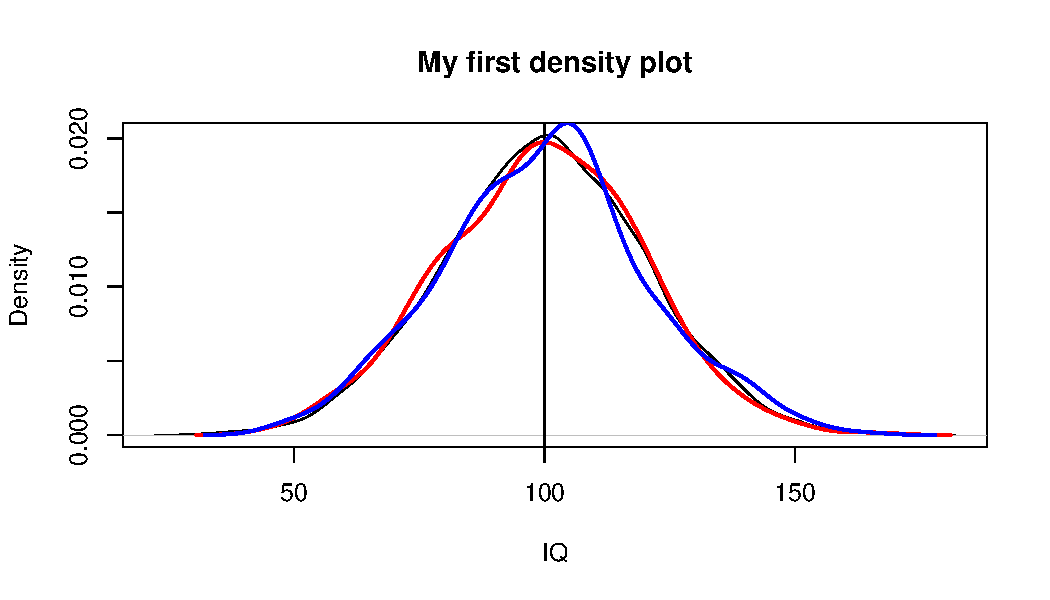
\includegraphics[width=\maxwidth]{figure/unnamed-chunk-14-1} 

\end{knitrout}
}
\end{frame}
%%%%%%%%%%%%%%%%%%%%%%%%%%%%%%%%%%%%%%%%%%%%%%%%%%%%%%%%%%%%%%%%%%%%%%%%%
\begin{frame}[fragile]{Simple Example on Sampling}{the sampling package}
%\frametitle{\vspace{-.05cm}\begin{center}\footnotesize{Simple Example on Sampling}\\ \scriptsize{the sampling package}\end{center}}
\footnotesize{
\begin{knitrout}
\definecolor{shadecolor}{rgb}{0.969, 0.969, 0.969}\color{fgcolor}\begin{kframe}
\begin{alltt}
\hlkwd{library}\hlstd{(sampling)}
\hlkwd{set.seed}\hlstd{(}\hlnum{42}\hlstd{)}
\hlstd{s.SRS1} \hlkwb{<-} \hlkwd{srswr}\hlstd{(}\hlnum{500}\hlstd{,}\hlkwd{nrow}\hlstd{(my.pop))}
\hlstd{s.SRSWOR1} \hlkwb{<-} \hlkwd{srswor}\hlstd{(}\hlnum{500}\hlstd{,}\hlkwd{nrow}\hlstd{(my.pop))}
\hlstd{my.samp.SRS1} \hlkwb{<-} \hlkwd{rbind}\hlstd{(my.pop[s.SRS1}\hlopt{!=}\hlnum{0}\hlstd{,],}
                      \hlstd{my.pop[s.SRS1}\hlopt{>}\hlnum{1}\hlstd{,])}
\hlstd{my.samp.SRSWOR1} \hlkwb{<-} \hlstd{my.pop[s.SRSWOR1}\hlopt{==}\hlnum{1}\hlstd{,]}
\end{alltt}
\end{kframe}
\end{knitrout}
}
\end{frame}
%%%%%%%%%%%%%%%%%%%%%%%%%%%%%%%%%%%%%%%%%%%%%%%%%%%%%%%%%%%%%%%%%%%%%%%%%%%%
\begin{frame}[fragile]{Simple Example on Sampling}{the sampling package}
%\frametitle{\vspace{-.05cm}\begin{center}\footnotesize{Simple Example on Sampling}\\ \scriptsize{the sampling package}\end{center}}
\begin{knitrout}
\definecolor{shadecolor}{rgb}{0.969, 0.969, 0.969}\color{fgcolor}\begin{kframe}
\begin{alltt}
\hlkwd{par}\hlstd{(}\hlkwc{mfrow} \hlstd{=} \hlkwd{c}\hlstd{(}\hlnum{1}\hlstd{,} \hlnum{2}\hlstd{))}
\end{alltt}
\end{kframe}
\end{knitrout}
\begin{minipage}{5.5cm}
\begin{knitrout}
\definecolor{shadecolor}{rgb}{0.969, 0.969, 0.969}\color{fgcolor}
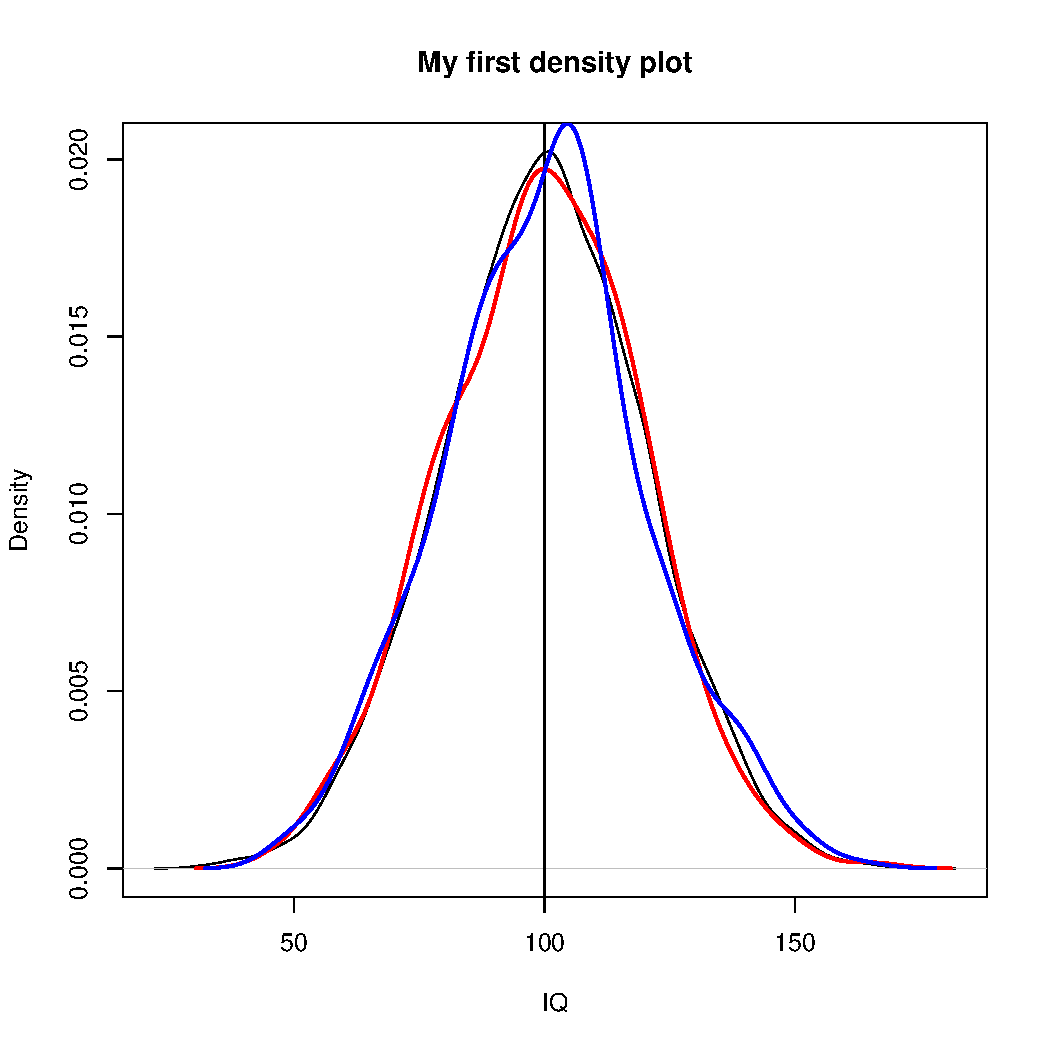
\includegraphics[width=\maxwidth]{figure/unnamed-chunk-17-1} 
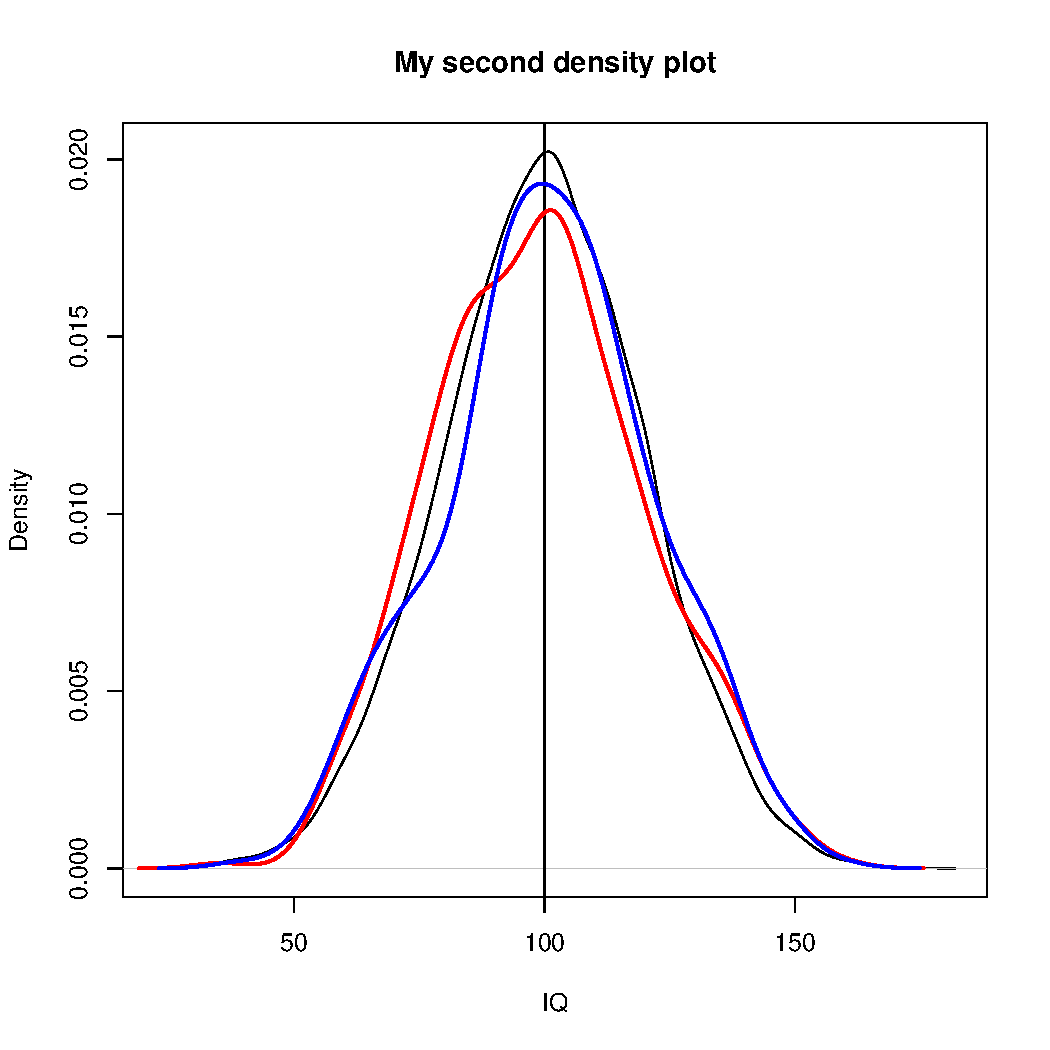
\includegraphics[width=\maxwidth]{figure/unnamed-chunk-17-2} 

\end{knitrout}
\end{minipage}
\begin{knitrout}
\definecolor{shadecolor}{rgb}{0.969, 0.969, 0.969}\color{fgcolor}\begin{kframe}
\begin{alltt}
\hlkwd{dev.off}\hlstd{()}
\end{alltt}
\end{kframe}
\end{knitrout}
\begin{itemize}
\pause\item should yield same results
\item[$\Rightarrow$] routine differs in "starting point"
\end{itemize}
\end{frame}
%%%%%%%%%%%%%%%%%%%%%%%%%%%%%%%%%%%%%%%%%%%%%%%%%%%%%%%%%%%%%%%%%%%%%%%%%%%
\begin{frame}[fragile]{Working Directory and Workspace}
%\frametitle{\vspace{-.05cm}\begin{center}\footnotesize{Working Directory and Workspace}\end{center}}
\footnotesize{
\begin{center}
\textbf{Declaring a working directory}\\
\end{center}
\R{path<-"H:/Sand\_ Summerschool/Data Day1/"\\
setwd(path)}}
\begin{itemize}
\footnotesize{
\item It is always useful to define and set your working directory at the beginning of each script
\item \R{getwd()} displays you your current working directory
\item \R{dir()} shows you all objects in a specific directory
\item \R{ls()} lists all objects in your workspace
\item \R{rm()} removes a object from your workspace
}
\end{itemize}
\footnotesize{
Example:\\
\begin{knitrout}
\definecolor{shadecolor}{rgb}{0.969, 0.969, 0.969}\color{fgcolor}\begin{kframe}
\begin{alltt}
\hlkwd{rm}\hlstd{(}\hlkwc{list} \hlstd{=} \hlkwd{ls}\hlstd{())}
\end{alltt}
\end{kframe}
\end{knitrout}
}

\end{frame}





%%%%%%%%%%%%%%%%%%%%%%%%%%%%%%%%%%%%%%%%%%%%%%%%%%%%%%%%%%%%%%%%%%%%%%%%%%%

\begin{frame}[fragile]{Reading and Writing Data}
%\frametitle{\vspace{-.05cm}\begin{center}\footnotesize{Reading and Writing Data}\end{center}}
\footnotesize{
\begin{center}
\textbf{Writing/ saving data and results}\\
\end{center}
\R{write.table(my.pop,"Synthetic Data Day1.csv",\\
            row.names = F, quote = F, dec = ".",sep = ",")}\\ 
            \textbf{OR:}\\
\R{save(my.samp.SRS,s.SRS,my.samp.SRSWOR1,file = "Day1.Rdata")}\\
\begin{itemize}
\item[$\Rightarrow$] See also: \R{write.csv} and \R{write.csv2} (\R{sep = }";")
\end{itemize}
\begin{center}
\textbf{Reading/ loading data and results}\\
\end{center}
\R{d1 <- read.table("Synthetic Data Day1.csv",\\
            header = F, dec = ".",sep = ",")}\\
            \textbf{OR:}\\
\R{load("Day1.Rdata")}}

\end{frame}
%%%%%%%%%%%%%%%%%%%%%%%%%%%%%%%%%%%%%%%%%%%%%%%%%%%%%%%%%%%%%%%%%%%%%%%%%%%
% \begin{frame}[fragile]{Exercise 1}
% %\frametitle{\vspace{-.05cm}\begin{center}\footnotesize{Exercise 1}\end{center}}
% \begin{exampleblock}{Sample sizes}
% \begin{enumerate}
% \item Generate 1000 numbers from a exponential distribution
% \item Draw three samples(n1=2,n2=10,n3=100)
% \item Plot the density and add the means of the three samples as vertical lines
% \end{enumerate}
% \end{exampleblock}
% \end{frame}
% %%%%%%%%%%%%%%%%%%%%%%%%%%%%%%%%%%%%%%%%%%%%%%%%%%%%%{Exercise 2}%%%%%%%%%%%%%%%%%%%%%%
% \begin{frame}[fragile]{Exercise 2}
% %\frametitle{\vspace{-.05cm}\begin{center}\footnotesize{Exercise 2}\end{center}}
% \begin{exampleblock}{Belgian municipalities/ variance decomposition}
% \begin{enumerate}\footnotesize{
% \item Load the dataset "belgianmunicipalities" from the \R{sample}-package using the \R{data()}-command 
% \item Inspect the structure of the dataset
% \item Calculate mean and variance of the variable \R{averageincome} 
% \item Calculate the mean of each province for that variable, plot your results and add the mean of \alert{3} 
% \item Recalculate the mean of \R{averageincome} based on the means by province and compare your results
% \item Make a boxplot of the variable \R{averageincome} for each province
% \item Calculate the variance of \R{averageincome} using variance decomposition and compare it with \alert{3}
% \begin{itemize}
% \item[$\Rightarrow$]\footnotesize{ Advice: consider the dataset as the aggregates for the whole population and use the formula for the population variance}
% \end{itemize}
% }
% \end{enumerate}
% \end{exampleblock}
% 
% \end{frame}
% 


\end{document}
